%%%%%%%%%%%%%%%%%%%%%%%%%%%%%%%%%%%%%%%%%%%%%%%%%%%%%%%%%%%%%%%%%%%%%%%%%%%%%%%%
%2345678901234567890123456789012345678901234567890123456789012345678901234567890
%        1         2         3         4         5         6         7         8

\documentclass[letterpaper, 10 pt, conference]{ieeeconf}  % Comment this line out
                                                          % if you need a4paper
%\documentclass[a4paper, 10pt, conference]{ieeeconf}      % Use this line for a4
                                                          % paper

\IEEEoverridecommandlockouts                              % This command is only
                                                          % needed if you want to
                                                          % use the \thanks command
\overrideIEEEmargins
% See the \addtolength command later in the file to balance the column lengths
% on the last page of the document



% The following packages can be found on http:\\www.ctan.org
%\usepackage{graphics} % for pdf, bitmapped graphics files
%\usepackage{epsfig} % for postscript graphics files
%\usepackage{mathptmx} % assumes new font selection scheme installed
%\usepackage{times} % assumes new font selection scheme installed
%\usepackage{amsmath} % assumes amsmath package installed
%\usepackage{amssymb}  % assumes amsmath package installed

\title{\LARGE \bf
Decentralised market-based strategy for cooperative multi-robot exploration 
}

%\author{ \parbox{3 in}{\centering autor1*
%         \thanks{*Use the $\backslash$thanks command to put information here}\\
%         Faculty of Electrical Engineering, Mathematics and Computer Science\\
%         University of Twente\\
%         7500 AE Enschede, The Netherlands\\
%         {\tt\small h.kwakernaak@autsubmit.com}}
%         \hspace*{ 0.5 in}
%         \parbox{3 in}{ \centering autor2**
%         \thanks{**The footnote marks may be inserted manually}\\
%        Department of Electrical Engineering \\
%         Wright State University\\
%         Dayton, OH 45435, USA\\
%         {\tt\small pmisra@cs.wright.edu}}
%}

\author{--% <-this % stops a space
%\thanks{*This work was not supported by any organization}% <-this % stops a space
\thanks{ All authors are with the University of Zagreb, Faculty of Electrical Engineering and Computing, LARICS Laboratory for Robotics and Intelligent Control Systems, Unska 3, 10000 Zagreb
 {\tt\small (nabrojati autore)}}%
%\thanks{$^{2}$P. Misra is with the Department of Electrical Engineering, Wright State University,
       % Dayton, OH 45435, USA
        %{\tt\small p.misra at ieee.org}}%
}


\begin{document}



\maketitle
\thispagestyle{empty}
\pagestyle{empty}


%%%%%%%%%%%%%%%%%%%%%%%%%%%%%%%%%%%%%%%%%%%%%%%%%%%%%%%%%%%%%%%%%%%%%%%%%%%%%%%%
\begin{abstract}

This work presents a novel approach to multi-robot exploration and mapping of an unknown area based on the market model. In the proposed approach exploration task has a weight that is a combination of cost, information gain and frontier occupancy function. Introduction of the frontier occupancy function in the weight causes mobile robots, members of multi-robot exploration team, to be more dispersed in the environment. During the negotiation process mobile robots exchange information on the weights of currently assigned tasks. The goal of negotiation process is to find tasks allocation that minimises weight of the group, hence minimising overall exploration time. Other factor the speeds up exploration process is related to the presented event-based communication that reduces amount of information exchange in negotiation process. The proposed strategy has been implemented in simulation environment and compared with a centralised market model method. The results of exploration demonstrate that the strategy distributes the mobile robots over an unknown area and enables quick mission accomplishment. 

\end{abstract}

 
%%%%%%%%%%%%%%%%%%%%%%%%%%%%%%%%%%%%%%%%%%%%%%%%%%%%%%%%%%%%%%%%%%%%%%%%%%%%%%%%
\section{INTRODUCTION}
Analysis and syntheses of decentralised multi-robot systems belong to core robotics problems that draw significant attention in last few decades. The coordination of a team of mobile robots that execute exploration missions of an unknown area is a common problem encountered in many applications, such as search and rescue \cite{rescue}, cleaning \cite{cleaning1}, \cite{cleaning2}, warehousing \cite{Wurman}, or planetary exploration \cite{planetary}, to number only few. Due to the fact that autonomous multi-robot systems are entering civil domain and as such will interact with people on daily basis, development of reliable coordination algorithms becomes inevitable.

In this paper, we consider the problem of an unknown area exploration with multiple mobile robots using the decentralised coordination strategy based on market model. Like in the human world, robots can be more effective when they work together. Moreover, a robot team can accomplish a predefined task much quicker than a single robot can \cite{free-market}. Another advantage of robot teams arises from possibility to merge overlapping sensor information, which in turn can help to compensate for sensor uncertainty \cite{segmentation}. Regarding the robustness of the system, using a multi-robot solution is the best option when a decentralised system is used. Even though the coordination is more difficult in this kind of systems \cite{Julia}, it is still easier then to get a group of uncoordinated individual robots to work together smoothly.
If done properly, coordination can lead to i) task accomplishment in the shortest possible time, ii) increased robustness, iii) higher map quality (in case of exploration task), and finally iv) the completion of tasks impossible for a single robot to perform \cite{survey-analysis}.

Different centralised and decentralised task allocation algorithms have been proposed by researchers \cite{Yamauchi}, \cite{burgard}, \cite{Simmons}, \cite{Sheng}, \cite{Konolige}. centralised task assignment for a multi-robot system is often not practical due to communication limits  \cite{free-market}, robustness issues \cite{survey-analysis}, time required for algorithm execution and scalability \cite{Julia}, but using a decentralised approach can mitigate some of these problems. In the centralised approach each robot has its own task that is assigned from a single central leader, using one of the centralised planning algorithm. The central leader communicates with each robot in order to receive an updated information about robot's pose and to assign a task to the robot after completion of a plan. Although achieving tight coordination typically requires that the mobile robots exchange large quantities of information about the environment and their current states, decentralised strategy proposed herein uses minimal information to ensure the negotiation in the market-model. It is assumed that communication between mobile robots is modelled by fully connected graph.  

Since the motivation was to achieve faster exploration and better cooperation between mobile robots, our market model insures that the mobile robots do not get too close to each other during the exploration. Moreover, the mobile robots are dispersed in the environment with the same goal, to accomplish the mission as fast as possible. If we image two mobile robots trying to reach the target point without cooperation, each of them will select the closest point to move to without considering what the other robot is doing. In order to avoid a conflicting assignment since both have selected the same task (Fig. \ref{fig:konflikt}), robot should cooperate. With cooperation robot Pioneer 1 will realize that robot Pioneer 2 is much closer to the first target point, and thus, better able to perform it. Similar problem is shown with UAVs in \cite{mit}. 

\begin{figure}[b!]
\minipage{0.16\textwidth}
  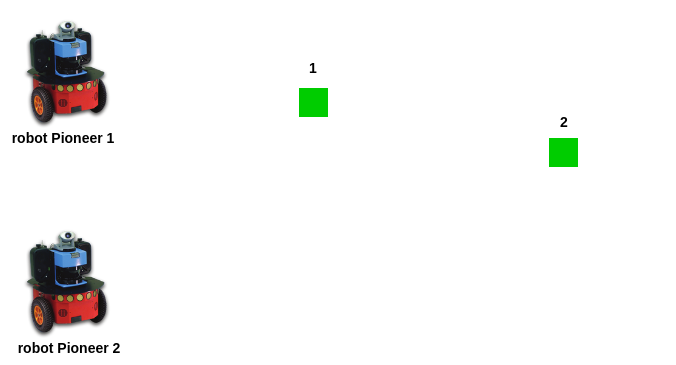
\includegraphics[width=\linewidth]{konflikt1.png}
\endminipage\hfill
\minipage{0.16\textwidth}
  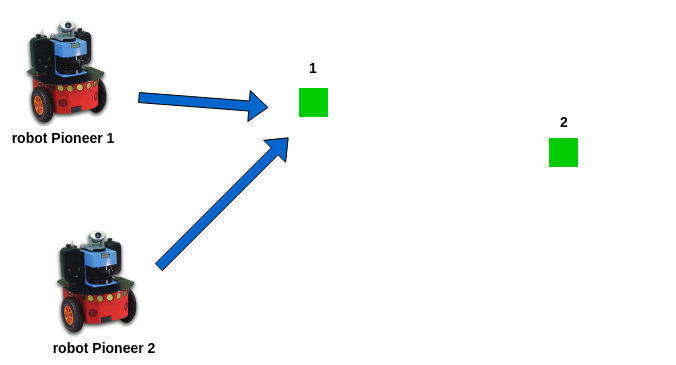
\includegraphics[width=\linewidth]{konflikt2.png}
\endminipage\hfill
\minipage{0.16\textwidth}%
  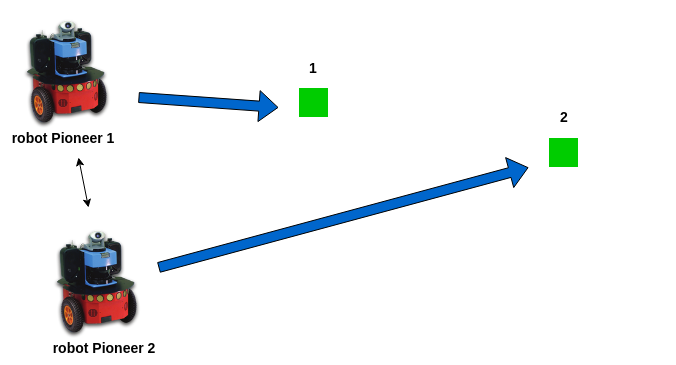
\includegraphics[width=\linewidth]{konflikt3.png}
\endminipage
\caption{Two mobile robots must reach the two target points. Without cooperation, assignments are conflicted and a task is left unassigned. By cooperating, the team of mobile robots is able to achieve higher mission performances.}
\label{fig:konflikt}
\end{figure}  


The rest of the paper is organised as follows. The related work is presented in the next section. In section III, an used exploration algorithm and a new exploration strategy based on market model is going to be explained. Simulation results are given in Section IV. In the final section conclusion will be given.



\section{RELATED WORK}


Previous studies of market-based models indicate that using central system for winner selection is not the best way for mobile robots coordination because this type of strategy (centralised approach) suffers from the single point of failure and, furthermore, it relies on complicated protocols \cite{Sheng}. Thus, several decentralised bidding models for coordination of multiple mobile robots have been proposed. 

Assigning robots to target points is achieved in different ways in the literature, for instance, with the nearest frontier approach \cite{Yamauchi}, the cost-utility approach \cite{burgard} or  with an exploration strategy based on a market economy \cite{market-economy}. Generally, these approaches aim to minimize the costs and maximize the utility and also mobile robots are updating the environment during the motion.  

Market-based multi-robot coordination approaches have been successfully implemented in centralised and decentralised ways.
centralised market-based algorithm described in \cite{burgard} improves robustness, but the negotiation process is complex because the coordination of mobile robots is performed by a central executive that creates a global map and executes auction with collected bids from the mobile robots, while in the same time assigning tasks according to the received bids. In other words, a robot (auctioneer) offers a task and other mobile robots compete by giving a bid. One with the highest revenue or the lowest cost is a winner. 

A special approach in which the number of mobile robots is greater then the number of candidate target points is presented by Hawley and Butler \cite{Hawley}. They implemented the auction-based coordination for both, task assignment and coalition formation. 
 
The general concept of market-based approaches is that the robots are independent in terms of planning for themselves, but are able to take into account team resources. It is shown in \cite{usporedba} that in case when different team sizes are included, the market method has an advantage over the centralised approach in terms of cost, and over the behavioral method in terms of computation time.
Hence, the proposed method is based on the market-model that includes an upgrade of the benefit function by adding the occupancy function which makes mobile robots more dispersed in the environment. Furthermore, the paper introduces a decentralised market-based strategy that implements event-based communication between mobile robots, thus reducing amount of information used in negotiation process. 




\section{APPROACH}
The previous work presented a multi-robot exploration system that can efficiently explore unknown terrain, and is robust to robot failures. Our approach attempts to accomplish these performances using strategy based on market model to coordinate the actions of the mobile robots. Action is defined as finished when the mobile robot reaches the desired point.  

\subsection{Goal point selection}
A global map of the environment is unknown at the moment when mobile robots start exploration. The goal is the environment mapping with mobile robots, that are supposed to communicate with each other. 
Nowadays a large number of algorithms for autonomous and coordinated exploration have been presented. Exploration algorithms can be intended weather for one robot or for a robot team. Some methods put whether emphasis on reducing research time or increasing the quality of the explored map, some have centralized, and some decentralized approach \cite{Julia}. This paper focuses on a multiple robot system in which mobile robots communicate with each other, share information of the explored area and negotiate. 

A popular basis for an unknown area exploration is the frontier-based exploration algorithm introduced by Yamauchi \cite{Yamauchi}. The idea is routing mobile robots to the frontier edges, lines that separate known space form unknown space in an occupancy grid map. The frontier edges detection is achieved using RRT (Rapidly Exploring Random Tree) algorithm developed by Hassan Umari and Shayok Mukhopadhyay \cite{Umari}. The RRT algorithm is not only biased towards unexplored regions, but also provides a general approach which can be extended to higher dimensional spaces.
In the frontier-based exploration mobile robot moves to the nearest frontier and explores new parts of the environment that are added to the map that is created during the exploration.
In addition, the mobile robots cooperate, since they share the acquired information, but their movements are uncoordinated. For instance, when the mobile robots are in close positions it is likely that they choose the same frontier to explore if no other coordination mechanisms are considered. However, the mobile robots can be coordinated such that they do not tend to move toward the same frontier cell \cite{burgard}. This approach is centralized since every robot constructs its bids and sends them to a central executive, that tries to maximize the total expected utility (information gain minus cost) of the mobile robots by assigning them tasks, based on their bids.  There is also a solution that takes into consideration only a distance cost for evaluating the goal assignment described in \cite{distance-cost}. 

In this paper we determine candidates for the goal locations using frontier-based approach with the expressions and functions that will be described in the next section. 

\subsection{Market-based strategy} 

At the core of our approach is negotiation between mobile robots during the exploration and mapping. The negotiation process is based on market model. The market model ensures coordination in our decentralized multi-robot system. The mobile robots exchange information under the assumption that all mobile robots communicate with each other and that in the process of negotiation each mobile robot takes into account the "statements" of the other mobile robots.

Every mobile robot $i$ get the list of frontier points from the RRT-based frontier detector module (Fig. \ref{fig:implementation-diagram}): 
\begin{equation}
   \boldsymbol{y}=\begin{bmatrix}
    \boldsymbol{y_{0}} & \boldsymbol{y_{1}} & \boldsymbol{y_{2}} & \hdots & \boldsymbol{y_{M}}
\end{bmatrix},
\end{equation}
where $M$ is  the number of frontier points, and every list member is a vector with $x$, $y$ and $z$ components. 
\begin{equation}
   \boldsymbol{y}=\begin{bmatrix}
   \begin{bmatrix}
           x_{0} \\
           y_{0} \\
           z_{0}
   \end{bmatrix}
    \begin{bmatrix}
         x_{1} \\
         y_{1} \\
         z_{1}
    \end{bmatrix}
    \begin{bmatrix}
         x_{2} \\
         y_{2} \\
         z_{2}
    \end{bmatrix}
    \hdots
    \begin{bmatrix}
         x_{M} \\
         y_{M} \\
         z_{M}
    \end{bmatrix}
\end{bmatrix}.
\end{equation}

In this paper we define the weight as a function of the cost, utility and frontier occupancy.  $i$ is an ordinal number of the mobile robot, and $j$ is an ordinal number of the frontier point. The cost function: $C_{ij}$: $R$ \(\rightarrow \text{$\mathbb{R}^{+}$}\) is a mapping from the set of resources $R$ to a positive real number. $C_{ij}$ describes the cost of $i$th robot to visit $j$th frontier point. The cost can be the function of the time, energy, but in our case the cost is the estimated distance traveled by robot to reach the target frontier point. The estimated distance is approximated using Euclidean distance between the position of mobile robot $\boldsymbol{p_{i}}$ and the frontier point position $\boldsymbol{q_{j}}$:
\begin{equation}\small
    C_{ij}=d(\boldsymbol{p_{i}}, \boldsymbol{q_{j}}) = \sqrt{(p_{ix}-q_{jx})^{2}+(p_{iy}-q_{jy})^{2}+(p_{iz}-q_{jz})^{2}}.
    \label{cost}
\end{equation}

The utility function $U_{ij}$:  \(\text{$\mathcal {M}$}\) \(\rightarrow \text{$\mathbb{R}^{+}$}\) returns a positive real number from the occupancy grid \(\text{$\mathcal {M}$}\). The cells of \(\text{$\mathcal {M}$}\) may be marked as free space, obstacle space, or unknown. The utility function is proportional to the number of unknown cells within a fixed distance from the frontier point $j$ in the previous defined radius $r$: 
\begin{equation}
    U_{ij} = \lambda_{u}c,
\end{equation}
where $\lambda_{u}$ is a constant experimentally determined, and  $c$ is the number of unknown cells within the circle radius $r$ and the circle center in the center of the frontier point. It is assumed that the mobile robot will detect all unknown cells around the assigned frontier point after reaching it. 

The frontier occupancy function $F_{ij}$ is 2-dimensional Gaussian function with the position of the peak in the frontier point and with the standard deviations $3\sigma_{x}=r_{f}$ and $3\sigma_{y}=r_{f}$. Moreover, the frontier occupancy function has a value if the frontier point $j$, for which mobile robot $i$ is calculating the weight, is in the range of radius $r_{f}$ from the position of the another robot assigned point ($q_{a}$). 

\begin{equation}
    F_{ij} =  \lambda_{f} e^{-\Big[\frac{(q_{jx} - q_{ax})^2}{2\sigma_{x}^2} + \frac{(q_{jy} - q_{ay})^2}{2\sigma_{y}^2}\Big]},
\end{equation}
where $\lambda_{f}$  is also  a constant experimentally determined. Fig. \ref{fig:radijusi} shows the example of the detected frontier point $j$ and its radii $r$ and $r_{f}$.

\begin{figure}[h!]
	\centering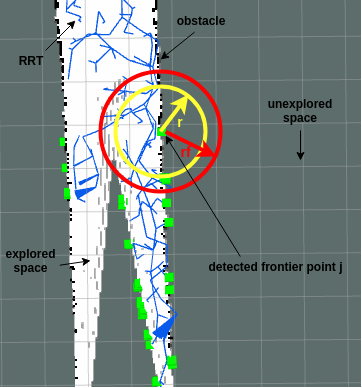
\includegraphics[width=0.8\columnwidth]{radius-and-space.png}
	\caption{Space definition, the detected frontier point $j$ and its radii $r$ and $r_{f}$.}
	\label{fig:radijusi}
\end{figure}

For each frontier point $j$ weight $W_{ij}$ $i$-th mobile robot is calculated as: 
\begin{equation}
   {W}_{ij}= {C_{ij}} - {U_{ij}} + {F_{ij}}.
   \label{weight}
\end{equation}

The weight matrix $\boldsymbol{W}$ ($N\times M$) is formed for $N$ mobile robots and $M$ received frontier points: 
\begin{equation}
    \boldsymbol{W} = \begin{bmatrix}
    W_{00} & W_{01} & \hdots & W_{0j} & \hdots & W_{0M}\\
    W_{10} & \ddots \\
    \vdots  \\
    W_{i0} \\
    \vdots \\
    W_{N0} &        &     &     &        &    W_{NM}
    \end{bmatrix}.
\end{equation}
Mobile robots exchange the information about the weight for the particular frontier point and make decisions for the future actions. Accordingly the amount of exchanging data is reduced, what result in easier and faster communication.
The weight matrix $\boldsymbol{W}$ represents the entry into the Hungarian algorithm which is able to find the optimal assignment solution in polynomial time \cite{hungarian}. 

Let matrix $X$ be matrix of zeros and ones, where $X[i,j]=1$ iff the frontier point $j$ is assigned to the mobile robot $i$.
Than the optimal task assignment has weight:
\begin{equation}
     {\mathrm{min}}\ \sum_{i} \sum_{j} W_{ij}\ X_{ij},
\end{equation}
sensing that minimization of sum could ensure the result as the Fig. \ref{fig:start} shows. 

\begin{figure}[t!]
	\centering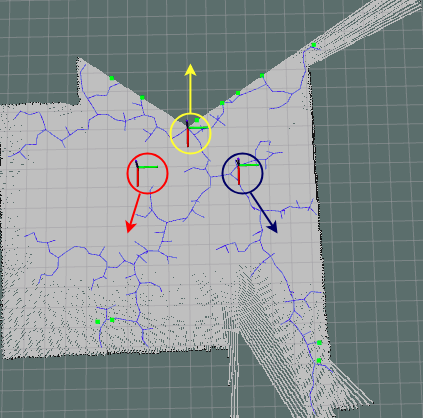
\includegraphics[width=0.9\columnwidth]{start.png}
	\caption {Decentralized strategy implemented on three mobile robots.}
	\label{fig:start}
\end{figure}

Our decentralized strategy is in progress during the robot's motion and there are seven steps for each robot to be executed (Algorithm \ref{algorithm1}).    

\begin{algorithm}[h!]
\caption{Decentralized strategy for a mobile robot $i$ exploration}
\label{algorithm1}
\begin{algorithmic}[1]
\For{ each frontier point $j$}
\State\hspace{\algorithmicindent} $W_{ij}$ = $C_{ij}$ - $U_{ij}$ + $F_{ij}$
\State\hspace{\algorithmicindent} Send $W_{ij}$ to the other mobile robots.
\State \hspace{\algorithmicindent} Receive the weights from the others.
\State \hspace{\algorithmicindent} Calculate weight matrix $\boldsymbol{W}$.
\State \hspace{\algorithmicindent} Hungarian algorithm ($\boldsymbol{W}$).
\State{\textbf{return} Frontier point is assigned to mobile robot $i$.}
\EndFor
\end{algorithmic}
\end{algorithm}

When the frontier point is assigned to mobile robot $i$ according to line 7 in Algorithm \ref{algorithm1}, the mobile robot starts path planning and tracking to the target frontier point. Moreover, at the moment when the mobile robot reach the goal, mission is over and a weight calculation request is sent to the others (Fig. \ref{fig:sustav3}). Besides request, current frontier point list $\boldsymbol{y}$ is sent and now the rest of robot team can execute first three steps of Algorithm \ref{algorithm1}.    

\begin{figure*}[t!]
    \centering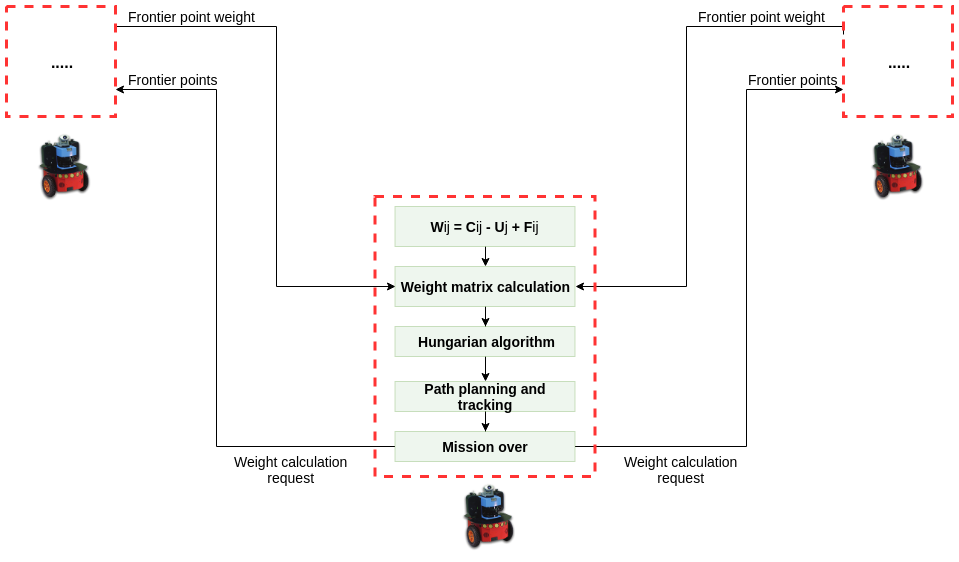
\includegraphics[width=0.7\textwidth,height=8cm]{structure.png}
	\caption{Implementation system of three mobile robots.}
    \label{fig:sustav3}
\end{figure*}


The weight matrix $\boldsymbol{W}$ is an entry to Hungarian algorithm and the described process is executing until the hole environment exploration. During the path planning and tracking simultaneous localization and mapping uses the laser and odometry data and closes the loop in the Fig. \ref{fig:implementation-diagram}.

\begin{figure}[H]
	\centering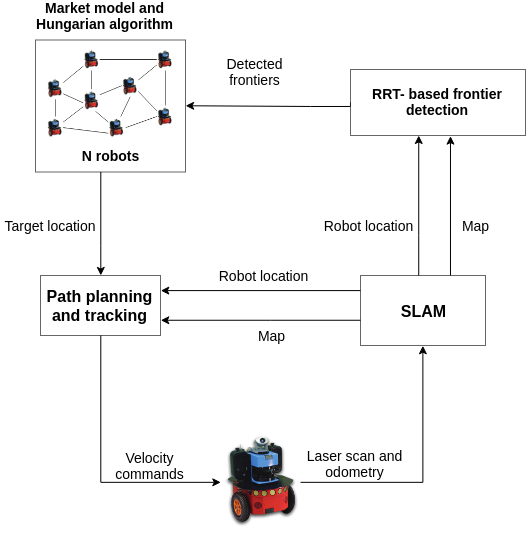
\includegraphics[width=1.0\columnwidth]{Impementationdiagram.png}
	\caption{Decentralized strategy diagram.}
	\label{fig:implementation-diagram}
\end{figure}



\begin{figure}[H]
	\centering
	\begin{minipage}{0.3\columnwidth}
		\centering
		
\includegraphics[width=\columnwidth]{free-space.png}
		\caption{(a)}
		\label{fig:free}
	\end{minipage}
	\begin{minipage}{0.3\columnwidth}
		\centering
		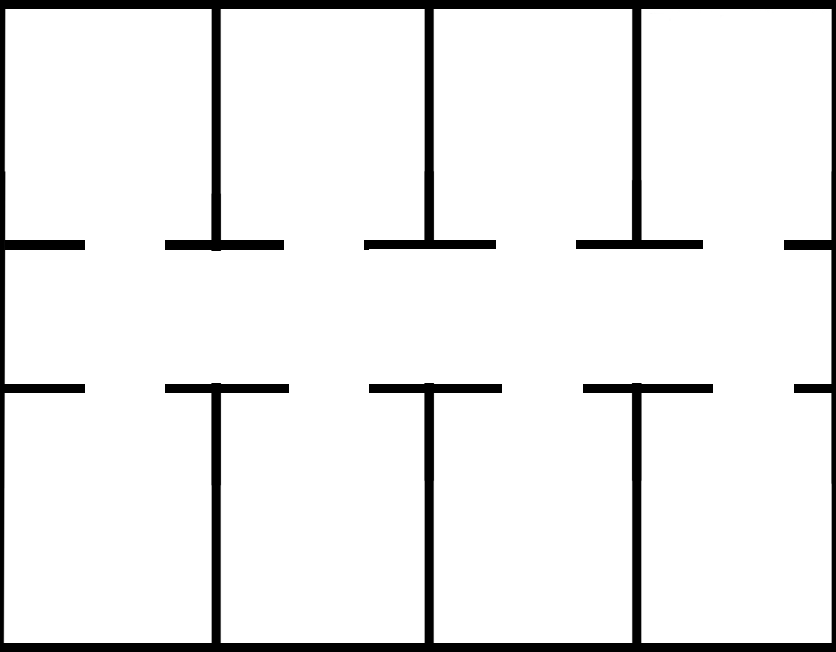
\includegraphics[width=\columnwidth]{office.png}
		\caption{(b)}
		\label{fig:office}
	\end{minipage}
	\begin{minipage}{0.3\columnwidth}
		\centering
		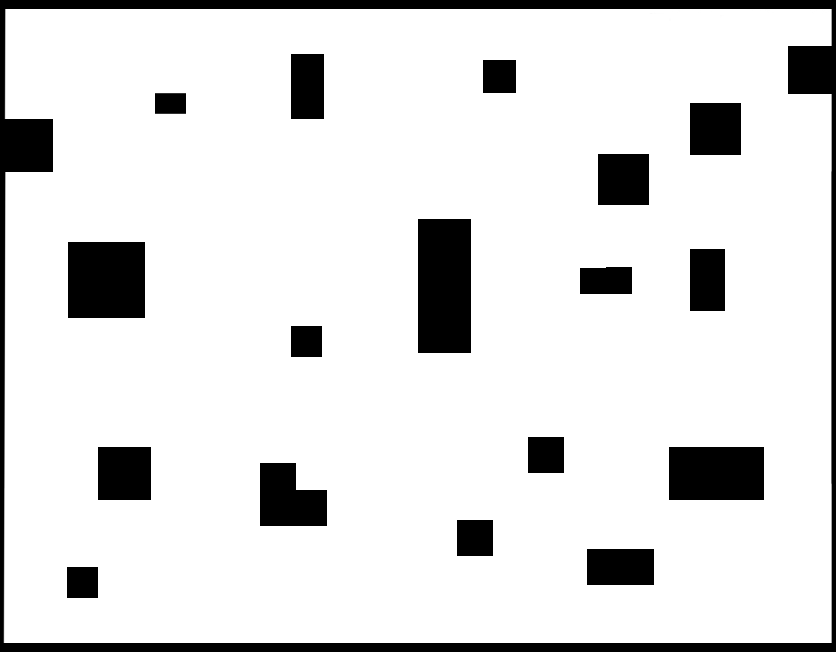
\includegraphics[width=\columnwidth]{unstructured.png}
		\caption{(c)}
		\label{fig:unstructured}
	\end{minipage}
 \caption{Simulation environments.}
 \label{fig:1}
\end{figure}

\section{SIMULATION RESULT}
The proposed strategy is implemented and tested using the Robot Operating System (ROS) framework.
Due to the fact that we want to show the efficiency of our decentralized strategy, we compared it with coordinated centralized market model described in \cite{burgard}. Expceriments were performed in the different indoor environments (Fig. \ref{fig:1}) with the number of robots from one to three. 

\newpage
\section{CONCLUSION}


\addtolength{\textheight}{-12cm}   % This command serves to balance the column lengths
                                  % on the last page of the document manually. It shortens
                                  % the textheight of the last page by a suitable amount.
                                  % This command does not take effect until the next page
                                  % so it should come on the page before the last. Make
                                  % sure that you do not shorten the textheight too much.

%%%%%%%%%%%%%%%%%%%%%%%%%%%%%%%%%%%%%%%%%%%%%%%%%%%%%%%%%%%%%%%%%%%%%%%%%%%%%%%%



\begin{thebibliography}{99}

\bibitem{fast-distributed} G. P. Das, T. M. McGinnity, S. A. Coleman, and L. Behera, A Fast Distributed Auction and Consensus Process Using Parallel Task Allocation and Execution, in Proceedings Irish Conf. Artificial Intelligence and Cognitive Science (AICS), pp. 244-253, 2011.

\bibitem{free-market} B. Dias, S. Stentz, A Free Market Architecture for Distributed Control of a Multirobot System, in 6th International Conference on Intelligent Autonomous Systems, pp. 115-122, 2000.

\bibitem{burgard} W. Burgard, M. Moors, C. Stachniss, and F. Schneider. Coordinated multi-robot exploration. IEEE Transactions on Robotics, 21(3):376–378, 2005.

\bibitem{Simmons} R. G. Simmons, D. Apfelbaum, W. Burgard, D. Fox, M. Moors, S. Thrun, and H. L. S. Younes, Coordination for Multi-Robot Exploration and Mapping, in Proceedings of the Seventeenth National Conference on Artificial Intelligence and Twelfth Conference on Innovative Applications of Artificial Intelligence, pp. 852-858, August 2000 

\bibitem{sold} B.P. Gerkey and M.J. Matarić, Sold!: Auction methods for multi-robot coordination. IEEE Transactions on Robotics and Automation,
18(5):758-768, 2002.

\bibitem{hungarian} H.W. Kuhn, The hungarian method for the assignment problem, Naval Research Logistics Quarterly, 2(1):83–97, 1955.

\bibitem{planetary} M.J. Matarić and G. Sukhatme, Task-allocation and coordination of
multiple robots for planetary exploration, in Proc. of the Int. Conf. on Advanced Robotics (ICAR), pages 61–70, Budapest, Hungary, 2001.

\bibitem{Yamauchi} B. Yamauchi, Frontier-based exploration using multiple robots, in
Proc. of the Second International Conference on Autonomous Agents, pages 47–53, Minneapolis, MN, USA, 1998.

\bibitem{market-economy} R. Zlot, A.T. Stenz, M.B. Dias, and S. Thayer, Multi-robot exploration controlled by a market economy, in Proc. of the IEEE Int. Conf. on Robotics and Automation (ICRA), Washington, DC, USA, 2002.

\bibitem{rescue} R. Murphy, Human-robot interaction in rescue robotics, IEEE Syst., Man, Cybern., C, Appl. Rev., vol. 34, no. 2, pp. 138–153, May 2004.

\bibitem{cleaning1} H. Endres, W. Feiten, and G. Lawitzky, Field test of a navigation system: autonomous cleaning in supermarkets, in Proc. IEEE Int. Conf. Robot. Autom. (ICRA), pp. 1779–1781, 1998.

\bibitem{cleaning2} P. Pinheiro, E. Cardozo, J. Wainer, and E. RohmerCleaning, Task Planning for an Autonomous Robot in Indoor Places with Multiples Rooms, International Journal of Machine Learning and Computing, Vol. 5, No. 2, April 2015.

\bibitem{segmentation} K. M. Wurm, C. Stachniss, and W. Burgard, Coordinated multi-robot exploration using a segmentation of the environment, in Proc. IEEE/RSJ  International Conference on Intelligent Robots and Systems (IROS), September 2008.

\bibitem{Julia} M. Julia, A. Gil, and O. Reinoso, A comparison of path planning strategies for autonomous exploration and mapping of unknown environments, Autonomous Robots, vol. 33, no. 4, pp. 427–444, 2012. 

\bibitem{indoor} C. Stachniss, O. M. Mozos, and W. Burgard, Efficient exploration of unknown indoor environments using a team of mobile robots, Annals of Mathematics and Artificial Intelligence, vol. 52, no. 2-4, pp. 205–227, 2008.

\bibitem{unsupervised-clustering} A. Solanas and M. A. Garcia, Coordinated multi-robot exploration through unsupervised clustering of unknown space, in Proc.  International Conference on Intelligent Robots and System (IROS), 2004.

\bibitem{comparison} M. Kulich, T. Juchelka, and L. Preucil, Comparison of exploration strategies for multi-robot search, Acta Polytech, 55(3):162, June 2015. 

\bibitem{survey-analysis} M. B. Dias, R. Zlot, N. Kalra,and A. Stentz, Market-based multirobot coordination: A survey and analysis, Proceedings of the IEEE 94 (7), 1257-1270, 2006.

\bibitem{mit} L. Brunet, Consensus-Based Auctions for Decentralized Task Assignment, Master thesis, Massachusetts Institute of Technology, June 2008.

\bibitem{Umari} H.Umari, and S. Mukhopadhyay, Autonomous Robotic Exploration Based on Multiple Rapidly-exploring Randomized Trees,  in Proc. IEEE/RSJ International Conference on Intelligent Robots and Systems (IROS), Vancouver, BC, Canada, September 2017.
  
\bibitem{Sheng} W. Sheng, Q. Yang, S. Ci, and N. Xi, Distributed Multi-robot Coordination Algorithm for Area Exploration and Mapping, IEEE International Conference on Robotics and Automation (ICRA) Workshop on The State-of-the-Art of Mobile Robot Area Coverage, 2004.

\bibitem{Konolige} D. Fox, J. Ko, K. Konolige, B. Limketkai, D. Schulz, and B. Stewart, Distributed Multirobot Exploration and Mapping, in Proceedings of the IEEE, vol. 94, no. 7, pp. 1325-1339, July 2016

\bibitem{usporedba} M. B. Dias, and A. Stentz, A Comparative Study between Centralized, Market-Based, and Behavioral Multirobot Coordination Approaches, in Proceedings of the 2003 IEEE/RSJ  International Conference on In Intelligent Robots and Systems (IROS), Las Vegas, Nevada, October 2003.

\bibitem{distance-cost} J. Faigl, M.Kulich, L.Preucil, Goal Assignment using Distance Cost in Multi-Robot Exploration, in Proc. IEEE/RSJ  International Conference on Intelligent Robots and Systems (IROS), Vilamoura, Algarve, Portugal, October 2012.

\bibitem{Hawley} J. Hawley, and Z. Butler, Hierarchical distributed task allocation for multi-robot exploration, in A. Martinoli, F. Mondada, N. Correll, G. Mermoud, M. Egerstedt, M. A. Hsieh, L. E. Parker, and K.Støy, Distributed autonomous robotic systems, vol. 83, pp. 445–458, Heidelberg: Springer, 2013.

\bibitem{Wurman} P. R. Wurman, R. D'Andrea, and M. Mountz, Coordinating hundreds of cooperative, autonomous vehicles in warehouses, in Proc. IAAI'07 Proceedings of the 19th national conference on Innovative applications of artificial intelligence, vol. 2, pp. 1752-1759, Vancouver, British Columbia, Canada, July 2007


\end{thebibliography}

\end{document}
